
\section{Deep Learning: Multi-layer Neural Networks}

% \subsection*{From Linear Models to NNs}
% - Linear prediction (with augmented features): $\quad y=f_{\operatorname{Lin}}(x)=\phi(x)^{\top} w$

% - Prediction with a neural network (NN): $y=f_{\mathbf{NN}}(x)=f(x)^\top w$


% \subsection*{Why Neural Networks?}
% - Classical machine learning:

% \begin{itemize}
%   \item Relatively simple models on top of features handcrafted by domain experts

%   \item Only works well when used with good handcrafted features

% \end{itemize}

% - Deep learning:

% \begin{itemize}
%   \item Large neural networks that learn features directly from the data

%   \item Can be viewed as a complicated feature extractor + linear prediction

%   \item Requires large amounts of data and compute to train

%   \item Quality often continues to improve substantially with more data and larger models

% \end{itemize}

% \subsection*{Recap: Logistic Regression}

% $f_{L R}(x)=p(1 \mid x)=\sigma\left(x^{\top} w+b\right)\\=\sigma\left(\sum_{i=1}^{d} x_{i} w_{i}+b\right)$

% where $\sigma(z)=(1+\exp (-z))^{-1}$ is the sigmoid

% - Pattern-matching perspective:

% \begin{itemize}
%   \item Task: classify between digit 1 and digit 0 using logistic regression

%   \item We learn a single pattern $w$ which we apply elementwise to each input $x$ (very restrictive!)

%   \item We classify the digit as 1 if $p(1 \mid x) \geq 0.5$ or, equivalently, if $\sum_{i=1}^{d} x_{i} w_{i} \geq-b$

% \end{itemize}

% \subsection*{Two-Layer Neural Networks}
% (aka two-layer perceptron)

% \begin{itemize}
%   \item Stack logistic regression units $\phi(x)_{j}=\sigma\left(\sum_{i=1}^{d} x_{i} w_{i, j}^{(1)}+b_{j}\right)$ (aka hidden units or neurons) in a hidden layer

%   \item Aggregate the hidden units using a linear function $\phi(x)^{\top} w^{(2)}$

% \end{itemize}

% \underline{Pattern-matching perspective:}

% \begin{itemize}
%   \item Task: classify between digit 1 and digit 0 with a two-layer neural network

%   \item Each hidden unit learns a different pattern (not necessarily interpretable!)

%   \item We classify based on a linear combination of these patterns $\Rightarrow$ much more flexible

% \end{itemize}

% \subsection*{Multi-layer Neural Networks}
% \includegraphics*[width=\columnwidth]{figures/nn1.png}

- Learnable Parameters: biases $\left\{b^{(l)}\right\}_{l \in[L]}$ and weights $\left\{\mathbf{W}^{(l)}\right\}_{l \in[L]}$ so we learn $\mathcal{O}\left(d K+K^{2} L\right) \approx \mathcal{O}\left(K^{2} L\right)$ parameters

% - Each column of $\mathbf{W}^{(l)}$ corresponds to the weights of one perceptron

% - Outputs of hidden layer $l$: $x^{(l)}=f^{(l)}\left(x^{(l-1)}\right):=\phi\left(\left(\mathbf{W}^{(l)}\right)^{\top} x^{(l-1)}+b^{(l)}\right)$

% \subsection*{Single Neuron View}
% \includegraphics*[width=\columnwidth]{figures/nn2.png}

% $
% x_{j}^{(l)}=\phi\left(\sum_{i=1}^{K} x_{i}^{(l-1)} w_{i, j}^{(l)}+b_{j}^{(l)}\right)
% $

% - Important: $\phi$ is non-linear otherwise we can only represent linear functions

% \subsection*{NNs extract features from the input}
% - NN = feature extractor + output layer

% - Feature extractor from $\mathbb{R}^{d}$ to $\mathbb{R}^{K}$ :

% - This function is defined by

% \begin{itemize}
%   \item The biases $\left\{b^{(l)}\right\}_{l \in[L]}$ and weights $\left\{\mathbf{W}^{(l)}\right\}_{l \in[L]}$ so we learn
% \end{itemize}

% $\Rightarrow O\left(d K+K^{2} L\right) \approx O\left(K^{2} L\right)$ parameters

% \begin{itemize}
%   \item The activation function $\phi$ we pick
% \end{itemize}

% - In practice: both $L$ and $K$ are large - overparametrized NNs

% \subsection*{Neural Network: Inference and Training}
% - $h(x)=f(x)^\top w^{(L+1)}+b^{(L+1)}$

% - Regression $h(x)$

% $
% \ell(y, h(x))=(h(x)-y)^{2}
% $

% - Binary Classification with $y \in\{-1,1\}$ $ \operatorname{sign}(h(x))$

% $
% \ell(y, h(x))=\log (1+\exp (-y h(x)))
% $

% - Multi-Class Classification with $y \in\{1, \ldots, K\}$
% $
% \operatorname{argmax}_{c \in\{1, \ldots, K\}} h(x)_{c}
% $

% $
% \ell(y, h(x))=-\log \frac{e^{h(x)_{y}}}{\sum_{i=1}^{K} e^{h(x)_{i}}}
% $

% \subsection*{Popular activation functions}
% \begin{itemize}
%   \item Sigmoid: $\phi(x)=\sigma(x)=\frac{1}{1+e^{-x}}$

%   \item $\operatorname{ReLU}: \phi(x)=(x)_{+}=\max \{0, x\}$

%   \item GELU: $\phi(x)=x \cdot \Phi(x) \approx x \cdot \sigma(1.702 x)$

% \end{itemize}

% \subsection*{Three theoretical questions in Deep Learning}
% \begin{itemize}
%   \item Expressive power of NNs: Why can neural networks approximate the functions we are interested in so effectively?

%   \item Success of naive optimization: Why does gradient descent consistently lead to a good local minimum?

%   \item Generalization miracle: Why don't neural networks overfit, despite having so many parameters?

% \end{itemize}

\subsection*{$L_{2}$ Approximation: Barron's result}
- Let $f: \mathbb{R}^{d} \rightarrow \mathbb{R}$ and define $\hat{f}(\omega)=\int_{\mathbb{R}^{d}} f(x) e^{-i \omega^{\top} x} d x$, its Fourier transform, $\int_{\mathbb{R}^{d}}|\omega||\hat{f}(\omega)| d \omega \leq C$ (smoothness assumption)

- \underline{Claim}: $\forall n \geq 1$, $r>0, \ \exists \ f_{n}$:
$
f_{n}(x)=\sum_{j=1}^{n} c_{j} \phi\left(x^{\top} w_{j}+b_{j}\right)+c_{0}
$,
s.t. 
$
\int_{|x| \leq r}\left(f(x)-f_{n}(x)\right)^{2} d x \leq \frac{(2 C r)^{2}}{n}
$
$\Rightarrow$ All sufficiently smooth function can be approximated by a one-hidden-layer NN

% \begin{itemize}
%   \item The more neurons allowed, the smaller the error.
%   \item The smoother the function (smaller $C$), the smaller the error
%   \item The larger the domain (the larger $r$), the greater the error
%   \item Approximation is in average (in $\ell_{2}$-norm)
%   \item Applicable for any "sigmoid-like" activation function
%   % \item The function $f_{n}$ is a one-hidden-layer $\mathrm{NN}$ with $n$ nodes $f_n =c^{\top} \phi\left(W^{\top} x+b\right)+c_{0}$
% \end{itemize}

\subsection*{$L_{1}$ Approximation}

% \begin{wrapfigure}{r}{0.4\columnwidth} 
%   \centering
%   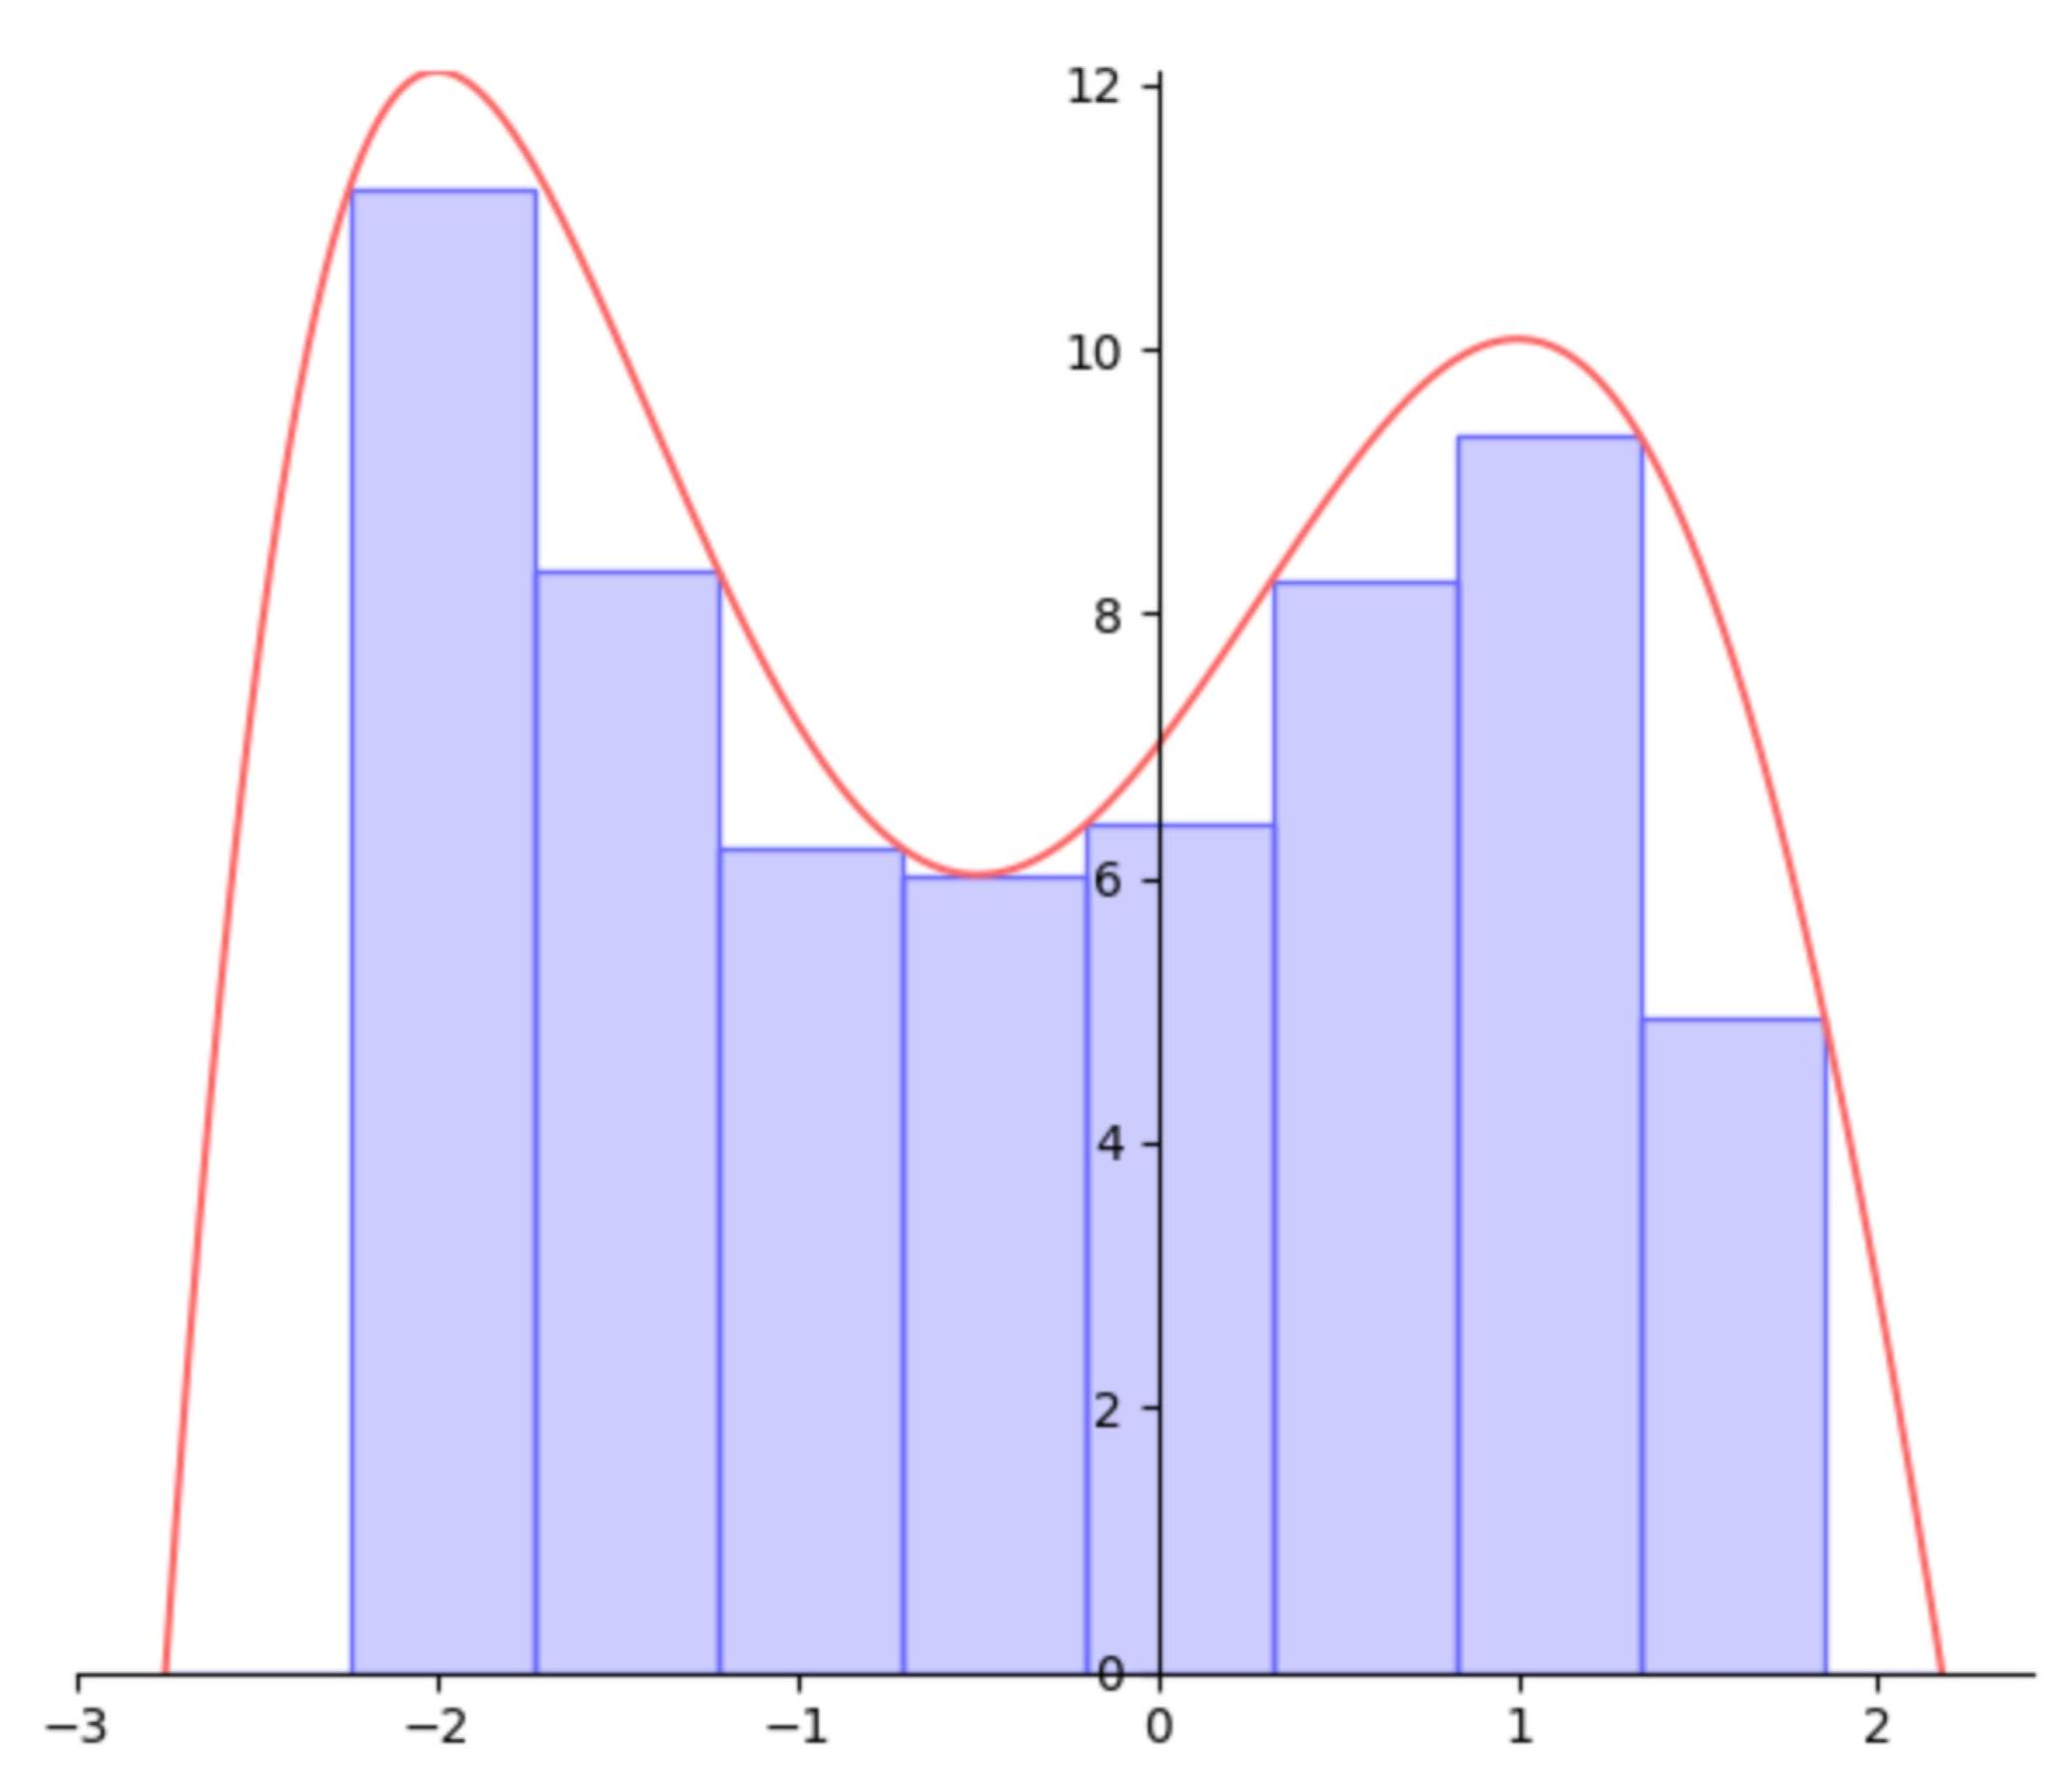
\includegraphics[width=0.4\columnwidth]{figures/nn3.jpg}
%   \vspace{-10pt}
% \end{wrapfigure}

% - ``A NN with sigmoid activation and at most two hidden layers can approximate well a smooth function in $\ell_{1}$-norm"

% - Approx in $\ell_{1}$-norm:
$
\int_{|x| \leq r}\left|f(x)-f_{n}(x)\right| d x \leq \text { Something small }
$


- $f: \mathbb{R} \rightarrow \mathbb{R}$ on a bounded domain, Riemann integrable - its integral can be approximated to any desired accuracy using "lower" and "upper" sums of the area of rectangles

- Approximation of the function by a sum of rectangle functions

$
\int_{|x| \leq r}\left|\color{red}{f(x)}\color{black}-\color{blue}{f_{n}(x)}\color{black}\right| d x 
=\int_{|x| \leq r}\left(\color{red}f(x)\color{black}-\color{blue}f_{n}(x)\color{black}\right) d x 
=\int_{|x| \leq r} \color{red}f(x)\color{black} d x-\int_{|x| \leq r} \color{blue}f_{n}(x) \color{black} d x 
=\int_{|x| \leq r} \color{red}f(x) \color{black}-\color{blue}\sum_{i} \text { Area(Rectangle }_{i})
$


\subsection*{Approximation of the rectangle}


- A rectangle function is equal to the sum of two step functions

- Approximate a step function with a sigmoid
$
\tilde{\phi}(x)=\phi(w(x-b))
$, 
% $b$ where the transition happens, $w$ makes the transition steeper


% Derivative: $\tilde{\phi}^{\prime}(b)=w / 4$
% $\Rightarrow$ The width of the transition is $O(4 / w)$

% $
% h(\phi(w(x-a))-\phi(w(x-b)))
% $


% \subsection*{Conclusion in the 1D case}
% \begin{enumerate}
%   \item Approximate the function in the Riemann sense by a sum of $k$ rectangles

%   \item Represent each rectangle using two nodes in the hidden layer of a neural network

%   \item Compute the sum of all nodes in the hidden layer (considering appropriate weights and signs) to get the final output

% \end{enumerate}

$\Rightarrow \mathrm{NN}$ with one hidden layer containing $2 k$ nodes for a Riemann sum with $k$ rectangles

% - Remarks:

% \begin{itemize}
%   \item The same intuition applies to any sigmoid-like function
%   \item This is an intuitive explanation, not a quantitative one
%   \item The weights $w$ must be large
% \end{itemize}


\subsection*{Larger dimension: $d=2$, same idea}
% Same idea:

% \begin{itemize}
%   \item Approximate the function by $2 \mathrm{D}$ rectangle functions
%   \item Approximate a 2D rectangle function by sigmoids
% \end{itemize}

- Two sigmoids can approximate an infinite rectangle function
% $\left(x_{1}, x_{2}\right) \mapsto \phi\left(w\left(x_{1}-a_{1}\right)\right)-\phi\left(w\left(x_{1}-b_{1}\right)\right)$

% The rectangle:

% \begin{itemize}
%   \item ranges from $a_{1}$ to $b_{1}$ in the $x_{1}$ direction
%   \item is unbounded in the $x_{2}$ direction

% \end{itemize}

% \subsection*{Two sigmoids can approximate an infinite rectangle function}
% $\left(x_{1}, x_{2}\right) \mapsto \phi\left(w\left(x_{2}-a_{2}\right)\right)-\phi\left(w\left(x_{2}-b_{2}\right)\right)$

% The rectangle:

% \begin{itemize}
%   \item ranges from $a_{2}$ to $b_{2}$ in the $x_{2}$ direction
%   \item is unbounded in the $x_{1}$ direction

% \end{itemize}
- Four sigmoids approximate a cross
% \subsection*{Four sigmoids approximate a cross}
% $\left(x_{1}, x_{2}\right) \mapsto \phi\left(w\left(x_{1}-a_{1}\right)\right)-\phi\left(w\left(x_{1}-b_{1}\right)\right)+\phi\left(w\left(x_{2}-a_{2}\right)\right)-\phi\left(w\left(x_{2}-b_{2}\right)\right)$

% $\Rightarrow$ This approximation is close to our objective, with the exception of the two infinite "arms"


% % How can we eliminate the crossed arms?

% \subsection*{Using the sigmoid to threshold unwanted infinite arms}
% Thresholding the function will eliminate the arms

% It is equivalent to composing it with $1_{y \geq c}$ for $c \in(1,2]$

% $\Rightarrow$ Approximate $1_{y \geq c}$ using a sigmoid with a large weight $w$ and an appropriate bias (e.g., $3 w / 2$ )


\subsection*{Point-wise approximations}
- Def: piecewise linear (PWL) function:

$
q(x)=\sum_{i=1}^{m}\left(a_{i} x+b_{i}\right) 1_{r_{i-1} \leq x<r_{i}} \text { with } a_{i} r_{i}+b_{i}=a_{i+1} r_{i}+b_{i+1}
$

- $\ell_{\infty}$-approximation result: Let $f$ be a continuous function on $[c, d]$. $\forall \ \varepsilon>0 \ \exists \ q \text{ s.t.}
\sup _{x \in[c, d]}|f(x)-q(x)| \leq \varepsilon
$


% \subsection*{Linear combinations of RELUs and PWL functions}
% $
% \sum_{i=1}^{m} \tilde{a}_{i}\left(x-\tilde{b}_{i}\right)_{+} \text {is a piecewise linear function }
% $

% How do we get a new segment with slope $a$ starting at $r>\max _{i}\left(\tilde{b}_{i}\right)$ ?

% Intuition: Get the kink at $r$ by setting $\tilde{b}_{i+1}=r$ and slope by additionally canceling existing slope i.e. $\tilde{a}_{i+1}=a-\sum_{i} \tilde{a}_{i}$


\subsection*{PWL functions can be written as combination of RELU}
- \underline{Claim} 1: Any PWL $q$ can be rewritten as
$
q(x)=\tilde{a}_{1} x+\tilde{b}_{1}+\sum_{i=2}^{m} \tilde{a}_{i}\left(x-\tilde{b}_{i}\right)_{+}
$
where $\tilde{a}_{1}=a_{1}, \tilde{b}_{1}=b_{1}, a_{i}=\sum_{j=1}^{i} \tilde{a}_{i}$ and $\tilde{b}_{i}=r_{i-1}$

- \underline{Claim} 2: $q$ can be implemented as a one-hidden-layer NN with RELU activation. Each term corresponds to one node:

% \begin{itemize}
%   \item Bias $-\tilde{b}_{i}$
%   \item Output weight $\tilde{a}_{i}$
% \end{itemize}

% The term $\tilde{a}_{1} x+\tilde{b}_{1}$ also corresponds to one node:

% \begin{itemize}
%   \item Bias $\tilde{b}_{1}$ : bias of the output node
% \end{itemize}



% \begin{itemize}
%   \item Term $\tilde{a}_{1} x=\tilde{a}_{1}(x)_{+}$since $x \in[0,1]$
% \end{itemize}

% \subsection*{\underline{Proof} of the equivalent formulation}

% $
% q(x)=\sum_{i=1}^{m}\left(a_{i} x+b_{i}\right) 1_{r_{i-1} \leq x<r_{i}} \quad r(x)=\tilde{a}_{1} x+\tilde{b}_{1}+\sum_{i=2}^{m} \tilde{a}_{i}\left(x-\tilde{b}_{i}\right)_{+}
% \tilde{a}_{1}=a_{1}, \tilde{b}_{1}=b_{1} \text { , } a_{i}=\sum_{j=1}^{i} \tilde{a}_{j} \text { , } \tilde{b}_{i}=r_{i-1}
% $

% \begin{itemize}
%   \item For $x \in\left[0, r_{1}\right]$
% \end{itemize}

% $
% \left(\tilde{a}_{1}, \tilde{b}_{1}\right)=\left(a_{1}, b_{1}\right) \Longrightarrow q(x)=a_{1} x+b_{1}=\tilde{a}_{1} x+\tilde{b}_{1}=r(x) \text { because } \tilde{b}_{2}=r_{1}
% $

% \begin{itemize}
%   \item For $x \in\left[r_{1}, r_{2}\right], r(x)=\tilde{a}_{1} x+\tilde{b}_{1}+\left(a_{2}-a_{1}\right)\left(x-r_{1}\right)_{+}$
% \end{itemize}

% $
% =a_{1} x+b_{1}+\left(a_{2}-a_{1}\right)\left(x-r_{1}\right)=a_{2} x+b_{1}-\left(a_{2}-a_{1}\right) r_{1}
% $

% $r^{\prime}(x)=a_{2}$ and $r\left(r_{1}\right)=q\left(r_{1}\right)$ as shown above

% $\Longrightarrow r(x)=q(x)$ for $x \in\left[r_{1}, r_{2}\right]$

% \subsection*{\underline{Proof} by induction}
% Let's assume that $r(x)=q(x)$ for $x \in\left[0, r_{i-1}\right]$

% For $x \in\left[r_{i-1}, r_{i}\right]$

% $
% \begin{aligned}
% r(x) & =\tilde{a}_{1} x+\tilde{b}_{1}+\sum_{j=2}^{m} \tilde{a}_{j}\left(x-\tilde{b}_{j}\right)_{+} \\
% & =\tilde{a}_{1} x+\tilde{b}_{1}+\sum_{j=2}^{i} \tilde{a}_{j}\left(x-\tilde{b}_{j}\right) \\
% & =\sum_{j=1}^{i} \tilde{a}_{j} x+\tilde{b}_{1}-\sum_{j=2}^{j} \tilde{a}_{j} \tilde{b}_{j}
% \end{aligned}
% $

% Thus

% \begin{itemize}
%   \item $r^{\prime}(x)=\sum_{j=1}^{i} \tilde{a}_{j}=a_{i}$ good slope
%   \item $r\left(r_{i-1}\right)=q\left(r_{i-1}\right)$ good starting point
% \end{itemize}



% $
% \Longrightarrow r(x)=q(x) \text { for } x \in\left[r_{i-1}, r_{1}\right]
% $

% Why: two affine functions with the same starting point and the same slope are equal

% \subsection*{Recap}
% \begin{itemize}
%   \item Neural networks consist of linear layers stacked together with non-linearities

%   \item A neural network can be seen as a learned feature extractor + a linear predictor

%   \item Neural networks typically require large amounts of data and compute to learn good features

%   \item Neural networks have very high representational power (i.e., the universal approximation result) in contrast to simple models like linear regression

% \end{itemize}